\chapter{Theoretic Background}
\label{chapters:TheoreticBackground}

In this chapter we will present some basic theoretic background.
All the concepts, cryptographic primitives, and ideas presented here are essential building blocks of the protocol proposed in this thesis.
As a result before someone carries on forward in this document, she should first have a basic understanding of this chapter.

\section{Symmetric Encryption}

The idea of symmetric encryption is quite simple.
We suppose that there exists an algorithm called $E$, which takes two inputs.
One input is a secret, called the key, and the other is some data we would like to encrypt.

Another algorithm called $D$ again takes two inputs and is the reverse of $E$.
This means that if we call $D$ with inputs the output of $E$ under some key $k$, and $k$ itself, the output will be the plaintext data. This is show in the below equation:

\[
  m = D(k, E(k, m))
\]

\section{Block Ciphers}

Block ciphers are a special case of symmetric encryption algorithms.
What makes them special is that they operate on a constant length block of data, hence the name.
While this constrain may appear very limiting, we will see that this is not the case.
In fact block ciphers have dominated the field of symmetric encryption.

The block cipher which is most commonly used is called AES, also known as Rijndael.
Its block size is 128 bits and depending on the AES version it has a key size of either 128, 192, or 256.

Exactly because AES is the most commonly used block cipher, it is also the most scrutinized and studied one.
Thus the crypto community is quite confident that AES is a secure construction, fully capable to be used for encrypted communications.

\section{Modes of Operation}

As we already stated, block ciphers operate on fixed chunks of data.
To overcome this limitation we need a mechanism so that we can break the plaintext in chunks of the cipher's block size, and then somehow apply the cipher in each chunk.
There are many modes of operation out there, but we will only talk about two of them.

One is called Electronic Code Book (ECB), and it is the naive solution that one can come up with when first tackling the problem at hand.
Suppose that we have a message $M$ which is a multiple of the block size.
We can then divide it into $n$ chunks $m_i$, each being one block in length:

\[
  M = m_1 || \dots || m_n
\]

Then we encrypt each block using the bloc cipher and the same key such that we get ciphertext $C$:

\[
  C = c_1 || \dots || c_n =  E(k,m_1) || \dots || E(k,m_n)
\]

It is easy to see that the decryption is trivial:

\[
  M = D(k, c_1) || \dots || D(k, c_n)
\]

However this has a crucial weakness.
You can easily see that if two chunks are the same then the resulting ciphertext will also be the same.
This might not seem important, but, believe us, it is detrimental to the mode's security.
Don't believe us yet? Here is an example:

\begin{figure}[h]
  \begin{minipage}{0.49\textwidth}
    
\includegraphics[scale=0.8]{Figures/Tux.jpg}
  \end{minipage}
  \begin{minipage}{0.49\textwidth}
    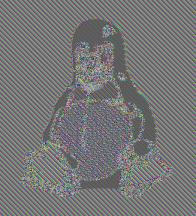
\includegraphics[scale=0.8]{Figures/Tux_ecb.jpg}
  \end{minipage}
  \caption[ECB in practice]{The image on the left is the plaintext. The image on the right is the plaintext encrypted with ECB mode. The plaintext image was created by Larry Ewing using GIMP.}
\end{figure}

The other is called Counter mode (CTR).
In this mode the block cipher itself does not encrypt the plaintext.
Instead it is used to produce a pseudo-random sequence of bits, in chunks equal to one block, which is then xor'ed with the plaintext.

To produce the $i$-th chunk $s_i$, it "encrypts" the number $i$ with the provided key.
As a result a bit stream is generated as shown below:

\[
  S = E(k, 1) || E(k, 2) || \dots || E(k, n)
\]

And the resulting ciphertext is:

\[
  C = m_1 \oplus s_1 || \dots || m_n \oplus s_n
\]

To decrypt, one can generate the same bit stream and xor it again with the ciphertext:

\[
  M = c_1 \oplus s_1 || \dots || c_n \oplus s_n
\]

Notice that this means that we use the encryption algorithm of the block cipher both for encryption and decryption.

Counter mode is a secure mode of operation suitable for use in production.
It also has a nice property called malleability, but more on that later.


\section{Message Integrity}

We now know how to keep a message secret.
Another major cryptographic problem is that of message integrity.
How can we be sure that a message we are reading came from who we think it did?

But why is this even necessary?
Since only the sender and the receiver have the secret key, only they should be able to construct valid ciphertexts.

Well, in general this is not correct.
Let's consider again the case of a block cipher used in CTR mode.
Remember that in this mode the block cipher is not directly used for encryption.
Instead it is used to generated a pseudorandom sequence of bits.
This sequence is then xor'ed to the plaintext and the result is the ciphertext.

Now let's see what will happen if a bit of the ciphertext is flipped, and we try to decrypt it.
Suppose $m_i$ and $c_i$ is the $i$-th bit of the plaintext and ciphertext respectively. $s_i$ is the $i$-th bit of the pseudorandom sequence produced during the CTR mode encryption process.
The follow relation holds:

\[
  m_i = c_i \oplus s_i
\]

Flipping a bit means taking its complement.
This means that the new plaintext bit $M_i$ will be:

\[
  M_i = c_i\prime \oplus s_i = (c_i \oplus s_i)\prime
\]

This means that an attacker could actually produce valid ciphertexts for plaintexts of his choosing by tampering with already sent messages!
This property is called malleability.

There are many more ways that an attacker could tamper with sent messages besides utilising the malleability properties of an encryption scheme.
This means that we need ways to authenticate our messages before we sent them.

\section{Hash Functions}

Before we tackle that problem we will have a look at hash functions.
These hash functions are algorithms that accept as input some data of arbitrary length and output some value of fixed length.

If this value is computed in such a way that the hash function $H$ satisfies the following properties (as stated in \cite{appliedcrypto}), then we call the function a \emph{cryptographic} hash function.

\begin{itemize}
  \item Pre-image resistance\\[0.2cm]
    For essentially any output value $h$ of the hash function $H$ it is computationally infeasible to find any input $x$ such that $H(x) = h$.

  \item Second pre-image resistance\\[0.2cm]
    For a given input $x$ it is computationally infeasible to find a second input $x\prime$ such that $x \ne x\prime$ and $H(x) = H(x\prime)$$x \ne x\prime$ and $H(x) = H(x\prime)$.

  \item Collision resistance\\[0.2cm]
    It is computationally infeasibly to find any pair of inputs $x$ and $x\prime$ such that $H(x) = H(x\prime)$\footnote{This and the previous property might seem the same, but notice that in the Second pre-image property $x$ is fixed, while in the collision resistance property it is not}.
\end{itemize}

Notice that collision resistance implies second pre-image resistance.
Likewise second pre-image resistance implies pre-image resistance.

\section{Message Authentication}

For the purpose of message authentication there are two main categories of solutions.
The first category uses a shared secret to create some sort of electronic signature for some data that we want to authenticate.
This type of signature is called a Message Authentication Code.

The second category uses a pair of keys, the private key, known only to the person signing the data, and the public key, known to everybody.
The public key is used to verify the signature.

\subsection{Message Authentication Codes (MAC)}

This case has many similarities with symmetric encryption.
Again we assume that there is a secret value, called the key, known only to the two parties communicating.
We also assume that an algorithm called $MAC$ exists which produces the signature, called the tag or mac.

This algorithm takes two inputs, the secret key $k$ and the message\footnote{This message can be plaintext or already encrypted} $m$ itself.
The algorithm works in a way such that the produced tag $t$ can only be calculated if you know $k$.

\[
  t = MAC(k, m)
\]

When the sending party wants to transmit a message, she calculates the tag and appends it to the message so that she sends $m||t$.
The receiving can recalculate the tag on his own.
He then checks if the appended tag is the same with the tag that he calculated.
If the two tags are the same then he accepts the message, otherwise he rejects it as it is probably tampered with.

\subsection{Public key signatures}

In this case we have two distinct algorithms.
On is called $Sign$ and is used to produce the signatures.
The other is called $Verify$ and is used to verify data.

The sender generates a tag $t$ using the $Sign$ algorithm:

\[
  t = Sign(priv, m)
\]

where $priv$ is the private key.
He then appends the tag to the message as in the MAC case and transmits $m||t$.

The receiving party then uses the $Verify$ algorithm.
This algorithm accepts as inputs the message $m$, the tag $t$, and the public key $pub$.
Its result is boolean, responding "YES" if the message is verified and "NO" if it is not:

\[
  result = Verify(m,t,pub)
\]

if $result$ is "YES" then she accepts the message. Otherwise she rejects it.

\section{Key Exchange Protocols (KEP)}

The goal of any key exchange protocol is to allow two users to agree on a secret value, known only to them, by exchanging some publicly known information.
This might be counter intuitive at first but as we will see in the next section this goal can be achieved with a very simple construction.

Basically a key exchange protocol is any mechanism that provides two functions.
One of them returns a tuple containing some private and some public information.
The public information returned by that function must be sent to the other so that he can calculate the secret value.
The other accepts the public values of the other user and the private values of this user.
It returns the secret value.

\begin{figure}[H]
  \begin{align*}
    <priv, pub> &= genkey() \\
    secret &= calculate\_secret(priv_i, pub_j)
  \end{align*}
  \caption[The interface of a Key Exchange Protocol]{The KEP interface. $pub_j$ is the public information of user $j$ and $priv_i$ the private information of user $i$.}
\end{figure}

\section{\dhname key exchange}

The \dhname key exchange is, as the name suggests, a key exchange protocol.
It plays a major role in our proposed protocol, since it is a building block of many of its components.
It was introduce by Whitfield Diffie and Martin Hellman in \cite{dhpaper}.

In this section we will examine how this KEP is constructed, and what public values must be exchanged.

First, we remind to the readers the operation of multiplication modulo a number, $\oplus$.
We want to multiply two numbers $a$ and $b$ modulo a number $n$, called "the modulo".
This means that we first multiply the two numbers as usual.
Then we calculate the remainder of the result when it is divided by the modulo.
This remainder is the result of the multiplication of those two numbers $a$, $b$ modulo $n$.
This means that if:

\[
  ab = np + r
\]

Then:

\[
  a \oplus b  = r
\]
.

In this section we will also symbolize:

\[
  a^x \equiv a \oplus \dots \oplus a = a^x \mod p
\]

These are all the maths needed to understand how the \dhname key exchange works.
To understand why it is also secure is a whole different matter and we will not cover it in this publication.

The \dhname construction supposes that the two users already agree on two values $g$ and $p$ which are publicly known.
The number $p$ must be prime and is called "the modulo" of the protocol.
The number $g$ is called the "generator" and has the property that for every number $k \in [1 \dots p-1]$ there exists a number $l$ in the same range such that $g^l = k$.

The private information for a user is any random integer $x$ such that $ 1 < x < p$.
The public information is $g^x \mod p$ (any exponentiation from now on will be modulo $p$).

The calculation of the shared secret is trivial.
A user $i$, with private information $x$, and public $g^x$, receives the public information $g^y$ of another user $j$.
He then calculates the value $s = (g^y)^x$ which is the shared secret.
Now note that with $i$'s public information, $j$ can also calculate the same value $s = (g^x)^y$.
The calculated value is the same for the two users since:

\[
  (g^y)^x = (g^x)^y = g^{xy}
\]

In algorithm \ref{algo:dh_genkey} we see the $genkey$ function, and in algorithm \ref{algo:dh_calculate_secret} the $calculate\_secret$ function.

From now on, the public and private information of a user will be called public and private keys accordingly.

\begin{algorithm}[h]
  \KwResult{The private and public information needed by the protocol}
  \Begin{
    x := $random_in_range(1,p-1)$

    p := $g^x$

    \Return{$<x, p>$}
  }
  \caption{The $genkey$ function}
  \label{algo:dh_genkey}
\end{algorithm}

\begin{algorithm}[h]
  \KwIn{$g^y$: the public value of the other user, $x$: the secret value of the user calling the function}
  \KwResult{The shared secret, which is known only to the two users}
  \Begin{
    \Return{$(g^y)^x$}
  }
  \caption{The $genkey$ function}
  \label{algo:dh_calculate_secret}
\end{algorithm}

\section{Person-in-the-Middle attacks}

\dhname is a great protocol for calculating shared secrets it has a grave disadvantage.
Consider the following scenario, where Mallory, an evil attacker can control the network so that she can read, drop, and inject packets:

User $i$ wants to privately communicate with user $j$.
She generates a private key $x$ and sends the public key $g^x$ to $j$.

Mallory interjects and copies and then drops the packet containing $i$'s public key.
She generates a private key $x\prime$ and the public counterpart $g^{x\prime}$.
She performs a \dhname exchange with $i$'s key and calculates $s_1 = g^{xx\prime}$, since she knows $x\prime$.
She then sends her public key to user $j$.

$j$ believes that the public key he just received belongs to $i$.
He generates his private key $y$, and sends the public key $g^y$ to $i$.
He also calculates $s_2 = g^{yx\prime}$ what he thinks is a shared secret known only to him and $i$.

Mallory interjects again to copy and drop the just sent package from the network.
She calculates $s_2 = g^{yx\prime}$, again she knows $x\prime$.
Then she sends her public key $g^{x\prime}$ to $i$, posing as $j$.

Now $i$ receives a public key which she thinks belongs to $j$.
Like $j$ she calculates the shared secret $s_1 = g^{xx\prime}$ which she thinks is only known between her and $j$.

\begin{figure}[h]
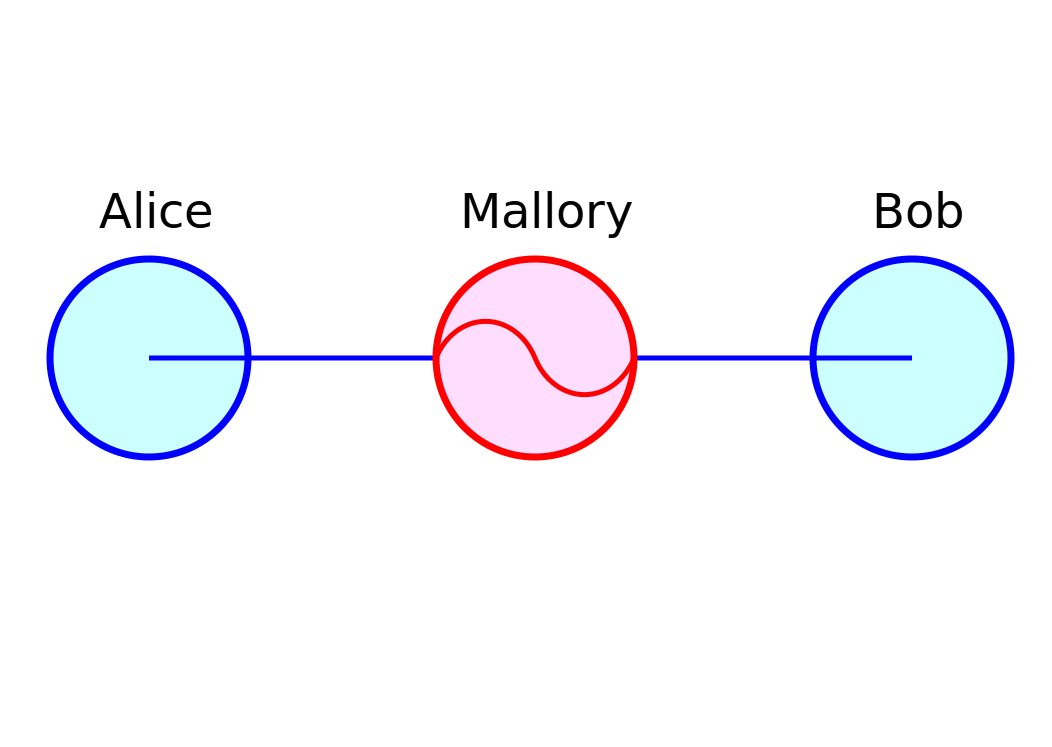
\includegraphics[scale=0.4]{Figures/Person_in_the_middle_attack.jpg}
\caption[A Person-in-the-Middle attack]{This figure demonstrates the situation just after Mallory has performed her Person-in-the-Middle attack.}
\end{figure}

The situation now is that $i$ and $j$ use two different secrets to communicate which are both known to Mallory.
Mallory can decrypt any message sent by $i$, for example, since she knows $s_i$.
She then can re-encrypt it using $s_2$ and relay it to $j$.

Nor $i$ neither $j$ will be able to know that such tampering is taking place and will continue to communicate, thinking that everything is fine.

The above scenario was described with the \dhname key exchange in mind.
However any similar situation where a malicious attacker can get between two communicating partners who think they are talking directly to each other is known as a Person-in-the-Middle attack.

\section{\tdhname key exchange}
\begin{figure}[h]
\begin{centering}
  \begin{tikzpicture}

  \def \dist {5cm}
  \def \longrad {1cm}
  \def \ephemrad {0.8cm}
  \def \sqrttwo {1.4142}

  \node[draw, circle, minimum size=\longrad] at (0,\dist) {$X$};
  \node[draw, circle, minimum size=\ephemrad] at (0,0) {$x$};
  \node[draw, circle, minimum size=\longrad] at (\dist,\dist) {$Y$};
  \node[draw, circle, minimum size=\ephemrad] at (\dist,0) {$y$};

  \draw[<->, >=latex] ({0 + (\sqrttwo * \longrad / 4)} ,{\dist  - (\sqrttwo * \longrad / 4)})
  -- ({\dist - (\sqrttwo * \ephemrad /4)},{0 + (\sqrttwo * \ephemrad / 4)});

  \draw[<->, >=latex] ({\dist - (\sqrttwo * \longrad / 4)} ,{\dist  - (\sqrttwo * \longrad / 4)})
  -- ({0 + (\sqrttwo * \ephemrad /4)},{0 + (\sqrttwo * \ephemrad / 4)});

  \draw[<->, >=latex] ({0 + \ephemrad/2}, 0) -- ({\dist - \ephemrad/2}, 0);

\end{tikzpicture}

  \caption[\tdhname in a picture]{These are the 3 \dhname key exchanges that are performed in this protocol}
\end{centering}
\end{figure}

\tdhname is another key exchange protocol.
It is an improvement of \dhname which introduces negligible overhead in the complexity of the protocol.
With doubling length of the first message containing the public keys of a user, this protocol provides both authentication and deniability.

\subsection{An Overview}

In this key exchange each user has a \dhname longterm keypair.
This should be authenticated to other users to exclude a person in the middle attack, like any other public key scheme.

When Alice wants to communicate with Bob, she generates an ephemeral \dhname key.
Suppose $X$ is her longterm private key and $x$ is her ephemeral private key.

She then sends the tuple $(g^X, g^x)$ to Bob, who upon receiving it does exactly what Alice did.
Supposing $Y$ is his longterm private key, he generates an ephemeral key $y$.
He then calculates the shared secret $s$ as shown below:

\[
  s = g^{Xy} || g^{xY} || g^{xy}
\]

Notice that an asymmetry exists, in the above calculation.
Should $g^Xy$ got first or should $g^{xY}$?
This can easily be decided by, for example, comparing the longterm public keys.
If $g^X > g^Y$ then:

\[
  s = g^{Xy} || g^{xY} || g^{xy}
\]

and if not:

\[
  s = g^{xY}|| g^{Xy} || g^{xy}
\]

And both users will calculate the same secret.

The shared secret generated by the above protocol is forward secret, and authenticated, yet deniable.

It is forward secret since even if someone forces Alice or Bob to hand over their long term secrets, the shared secret cannot be reconstructed.
This is true because to calculate the shared secret, either $x$ or $y$ are needed, and we assume that ephemeral secrets are destroyed after a session finishes.

It is authenticated since to calculate the above secret one needs to know either $X$ or $Y$.

It is deniable since the only values exchanged during the protocol are public keys.

\subsection{The catch}

There is a catch however. Suppose Eve would like to be able to read \emph{some} message that Alice has authored and sent to Bob.
What she can do is create an "ephemeral" key $e$.
She then starts a conversation with Alice, posing as Bob.
Alice might respond, create the shared secret and start communicating.
Eve does NOT know the shared secret, so she cant read any messages or prove anything, but she might be able to calculate it in the future.

If Eve at some point forces Bob to hand over his long term secrets then she can recreate the shared secret.
She can thus read the first message that Alice has tried to sent to "Bob" using the shared secret calculate with the phony ephemeral.
This is possible since she now knows $Y$ (bob's longterm secret) and she also knows $e$.
This breaks the forward secrecy of the protocol.

This can be easily solved if both Alice and Bob first make sure that they have both arrived at the same shared secret.

Suppose that Alice has calculated the shared secret $s$. She uses that secret to send an encrypted and authenticated message to Bob.
That message contains data known to everybody, the word "confirmation" for example.
She won't send any further messages unless she receives the same confirmation message from Bob.

On receiving the confirmation message Bob can be sure that Alice has calculated the shared secret.
He then sends a confirmation message himself, so that Alice too can be sure that Bob has calculated the shared secret.

\section{Message Ordering}

One difficulty that multi-party chat protocols need to overcome is that of message ordering.
This is confusing at first.
Why would the ordering of the messages be so important?
If a conversation is reordered it shouldn't make any sense.

Unfortunately this is not the case.
To illustrate why message order is important we will examine the so called "ice cream attack".

Suppose that Alice, Bob, and Mallory are chatting in one chat room.
Mallory wants to make Alice believe that Bob is a dangerous criminal.
We assume that she has significant control over the network and can delay packages.
To achieve her gaol she does the following:

She sends the message "Who wants some ice cream?" in the chat room.
But she delays the package going to Alice, so that Alice does not receive it yet.
Bob will obviously reply that he wants ice cream.
Let's suppose he sends the message "I do".
Again Mallory will put the package on hold before she delivers it to Alice.
And finally she transmits the message "Who wants to do something illegal?", which she allows to be delivered to both Alice and Bob.
She then allows Bob's message, saying "I do", to go through to Alice.
After that she also allows her original message, saying "Who wants some ice cream?" to also go to Alice.

Now, what did Alice actually see?
First, she saw that Mallory asked who wanted to do something illegal.
And then she saw Bob saying that he does!
In her eyes, bob is willing to do engage in illegal activities.
Maybe she shouldn't hang out with him any more.

And that exactly is the "ice cream attack".
Can multi-party chat protocols defend against such vulnerabilities?
The problem at hand is generally still open and goes beyond the scope of this publication.
However at section \ref{chapters:FutureWork} we shall briefly examine a proposed solution which is compatible to our protocol.
